% This example is meant to be compiled with lualatex or xelatex
% The theme itself also supports pdflatex
\PassOptionsToPackage{unicode}{hyperref}
\documentclass[aspectratio=1610, 12pt, xcolor=dvipsnames]{beamer}

% Warning, if another latex run is needed
% \usepackage[aux]{rerunfilecheck}

% just list chapters and sections in the toc, not subsections or smaller
\setcounter{tocdepth}{1}

%------------------------------------------------------------------------------
%------------------------------ Fonts, Unicode, Language ----------------------
%------------------------------------------------------------------------------
\usepackage{fontspec}
\defaultfontfeatures{Ligatures=TeX}  % -- becomes en-dash etc.

% german language
\usepackage{polyglossia}
\setdefaultlanguage{german}

% for english abstract and english titles in the toc
\setotherlanguages{english}

% intelligent quotation marks, language and nesting sensitive
\usepackage[autostyle]{csquotes}

% microtypographical features, makes the text look nicer on the small scale
\usepackage{microtype}

% colors and stuff
\usepackage{xcolor}
\usepackage[most]{tcolorbox}
% Here was colback=SpringGreen before but it is not finding the xcolor package
\tcbset{on line,
        boxsep=4pt, left=0pt,right=0pt,top=0pt,bottom=0pt,
        colframe=white,colback=green,
        highlight math style={enhanced}
        }
\newtcolorbox{mybox}[3][]
{
  colframe = #2!25,
  colback = #2!20,
  coltitle = #2!20!black,
  title = {#3},
  #1
}
%\colorlet{Green!40}
%------------------------------------------------------------------------------
%------------------------ Math Packages and settings --------------------------
%------------------------------------------------------------------------------

\usepackage{amsmath}
\usepackage{amssymb}
\usepackage{mathtools}
\usepackage{bbold}

% Enable Unicode-Math and follow the ISO-Standards for typesetting math
\usepackage[
  math-style=ISO,
  bold-style=ISO,
  sans-style=italic,
  nabla=upright,
  partial=upright,
]{unicode-math}
\setmathfont{Latin Modern Math}

% nice, small fracs for the text with \sfrac{}{}
\usepackage{xfrac}


%------------------------------------------------------------------------------
%---------------------------- Numbers and Units -------------------------------
%------------------------------------------------------------------------------

\usepackage[
  locale=DE,
  separate-uncertainty=true,
  per-mode=symbol-or-fraction,
]{siunitx}
\sisetup{math-micro=\text{µ},text-micro=µ}
% \sisetup{tophrase={{ to }}}
%------------------------------------------------------------------------------
%-------------------------------- tables  -------------------------------------
%------------------------------------------------------------------------------

\usepackage{booktabs}       % \toprule, \midrule, \bottomrule, etc

%------------------------------------------------------------------------------
%-------------------------------- graphics -------------------------------------
%------------------------------------------------------------------------------

\usepackage{graphicx}
%\usepackage{rotating}
\usepackage{grffile}
\usepackage{tikz}
\usepackage{circuitikz}
\usepackage{tikz-feynman}
\usepackage{subcaption}

% allow figures to be placed in the running text by default:
\usepackage{scrhack}
\usepackage{float}
\floatplacement{figure}{htbp}
\floatplacement{table}{htbp}

% keep figures and tables in the section
\usepackage[section, below]{placeins}

% smileys
\usepackage{MnSymbol,wasysym}

%------------------------------------------------------------------------------
%---------------------- customize list environments ---------------------------
%------------------------------------------------------------------------------

\usepackage{enumitem}
\usepackage{listings}
\usepackage{hepunits}

\usepackage{pdfpages}
%------------------------------------------------------------------------------
%------------------------------ Bibliographie ---------------------------------
%------------------------------------------------------------------------------

\usepackage[
  backend=biber,   % use modern biber backend
  autolang=hyphen, % load hyphenation rules for if language of bibentry is not
                   % german, has to be loaded with \setotherlanguages
                   % in the references.bib use langid={en} for english sources
]{biblatex}
\addbibresource{references.bib}  % the bib file to use
\DefineBibliographyStrings{german}{andothers = {{et\,al\adddot}}}  % replace u.a. with et al.


% Load packages you need here
% \usepackage{polyglossia}
% \setmainlanguage{german}

\usepackage{csquotes}


% \usepackage{amsmath}
% \usepackage{amssymb}
% \usepackage{mathtools}

\usepackage{hyperref}
\usepackage{bookmark}

% load the theme after all packages

\usetheme[
  showtotalframes, % show total number of frames in the footline
]{tudo}

% Put settings here, like
\unimathsetup{
  math-style=ISO,
  bold-style=ISO,
  nabla=upright,
  partial=upright,
  mathrm=sym,
}

% \setbeamertemplate{itemize item}{\scriptsize$\blacktriangleright$}
% \setbeamertemplate{itemize subitem}{\scriptsize$\blacktriangleright$}

%Titel:
\title{Bachelorseminar: Detektorsysteme des LHCb und Hardwareprojekte}
%Autor
\author[N.Breer]{\textbf{Nils Breer}}
%Lehrstuhl/Fakultät
\institute{TU Dortmund}
%Titelgrafik muss ich einfueren!!!
%\titlegraphic{\includegraphics[width=0.3\textwidth]{content/Bilder/interferenz.jpg}}
\date{18.04.2023}

\begin{document}
\maketitle

\begin{frame}\frametitle{Vertex Locator (VELO)}
  \begin{columns}
    \begin{column}[c]{0.48\textwidth}
      \begin{itemize}
        \item $\bullet$\, 30 $\si{\micro\metre}$ räumliche Auflösung
        \item $\bullet$\, Effizienz zur PV Findung \approx 90\%
        \item $\bullet$\, 52 Module, 4 Hybride Pixel Sensoren, 26 pro Seite
        \item $\bullet$\, mechanische Verschiebung der Seiten möglich je nach Beam Qualität
        \item $\bullet$\, RF Folie separiert Vakuum der Strahlröhre vom VELO
        \item $\bullet$\, Vertexauflösung maximal bei minimalem Abstand zur Strahlröhre
      \end{itemize}
    \end{column}
    \begin{column}[c]{0.48\textwidth}
      \begin{figure}
        \centering
        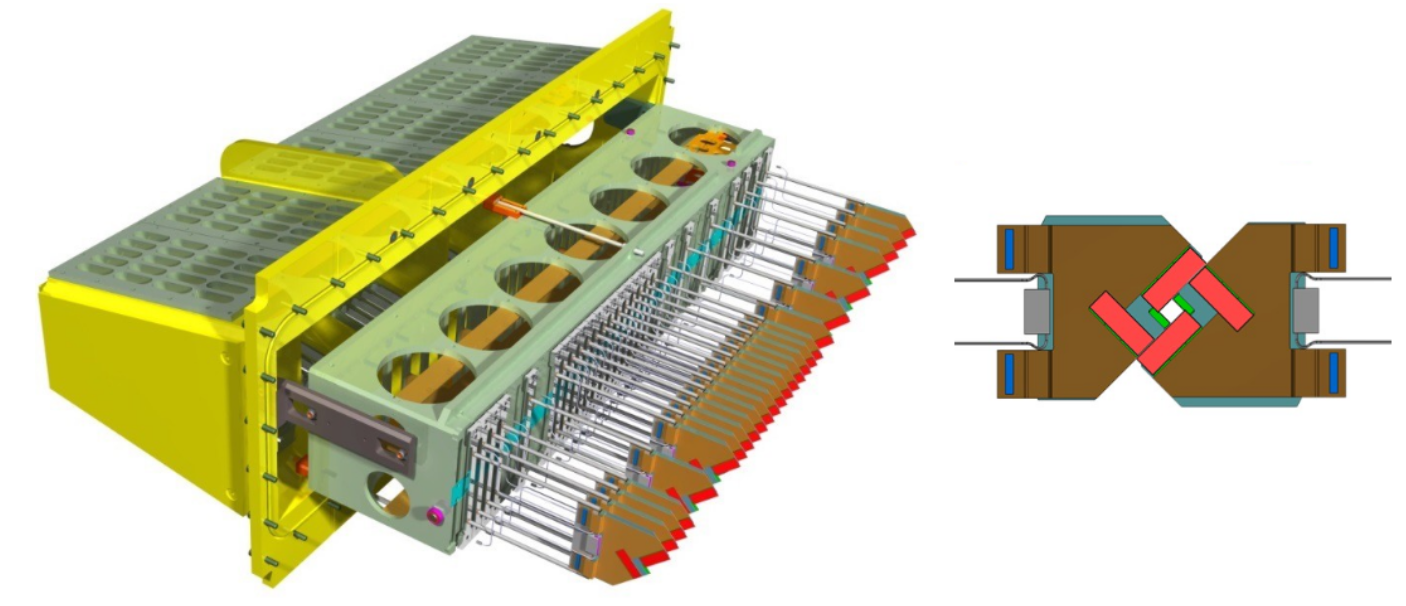
\includegraphics[width=\textwidth]{plots/velo.png}
      \end{figure}
    \end{column}
  \end{columns}
\end{frame}

\begin{frame}\frametitle{Warum ist der VELO so interessant/wichtig}
  \begin{columns}
    \begin{column}[c]{0.48\textwidth}
      \begin{itemize}
        \item $\bullet$\, Vollständige Rekonstruktion von Teilchen Trajektorien
        \item $\bullet$\, Upstream vom Magnet \to Interessante Wechselwirkungen zur B-Physik können teils vorselektiert werden
      \end{itemize}
    \end{column}
    \begin{column}[c]{0.48\textwidth}
      RF Folie und ihre Wichtigkeit:
      \begin{itemize}
        \item $\bullet$\, LHC kann die Elektronik des VELO stören \to verhindert Radiofrequenzen
        \item $\bullet$\, Störfelder werden abgeleitet um den Strahl nicht zu beeinflussen
        \item $\bullet$\, Verhindert "outgassing" aus VELO Bauteilen in das Beam Pipe Vakuum
      \end{itemize}
    \end{column}
  \end{columns}
\end{frame}

\begin{frame}\frametitle{Der Upstream Tracker (UT)}
  \begin{columns}
    \begin{column}[c]{0.48\textwidth}
      \begin{itemize}
        \item $\bullet$\, 4 Silizium Detektorplatten
        \item $\bullet$\, $X-U-V-X$ stereo Aufbau
        \item $\bullet$\, U, V um \pm 5 grad gedreht \to räumliche 2D Auflösung wichtig für Auflösung in y + Unterdrückung von "ghost hits" welche nicht zuzuordnen sind
        \item $\bullet$\, integrierte B-feldstärke: 4 Tm \to Impulsebestimmung zur Spurrekonstruktion und Triggerentscheidungen
      \end{itemize}
    \end{column}
    \begin{column}[c]{0.48\textwidth}
      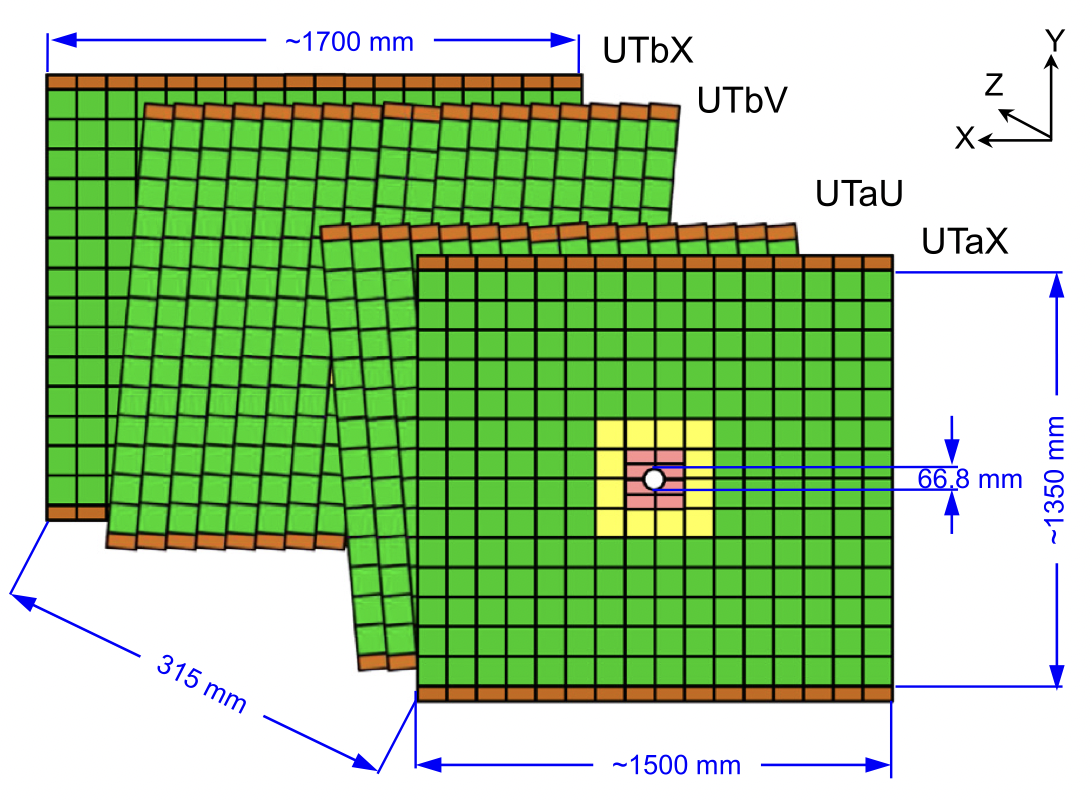
\includegraphics[width=\textwidth]{plots/UT.png}
    \end{column}
  \end{columns}
\end{frame}

\begin{frame}\frametitle{Upstream Tracker importance}
  \begin{columns}
    \begin{column}[c]{0.48\textwidth}
      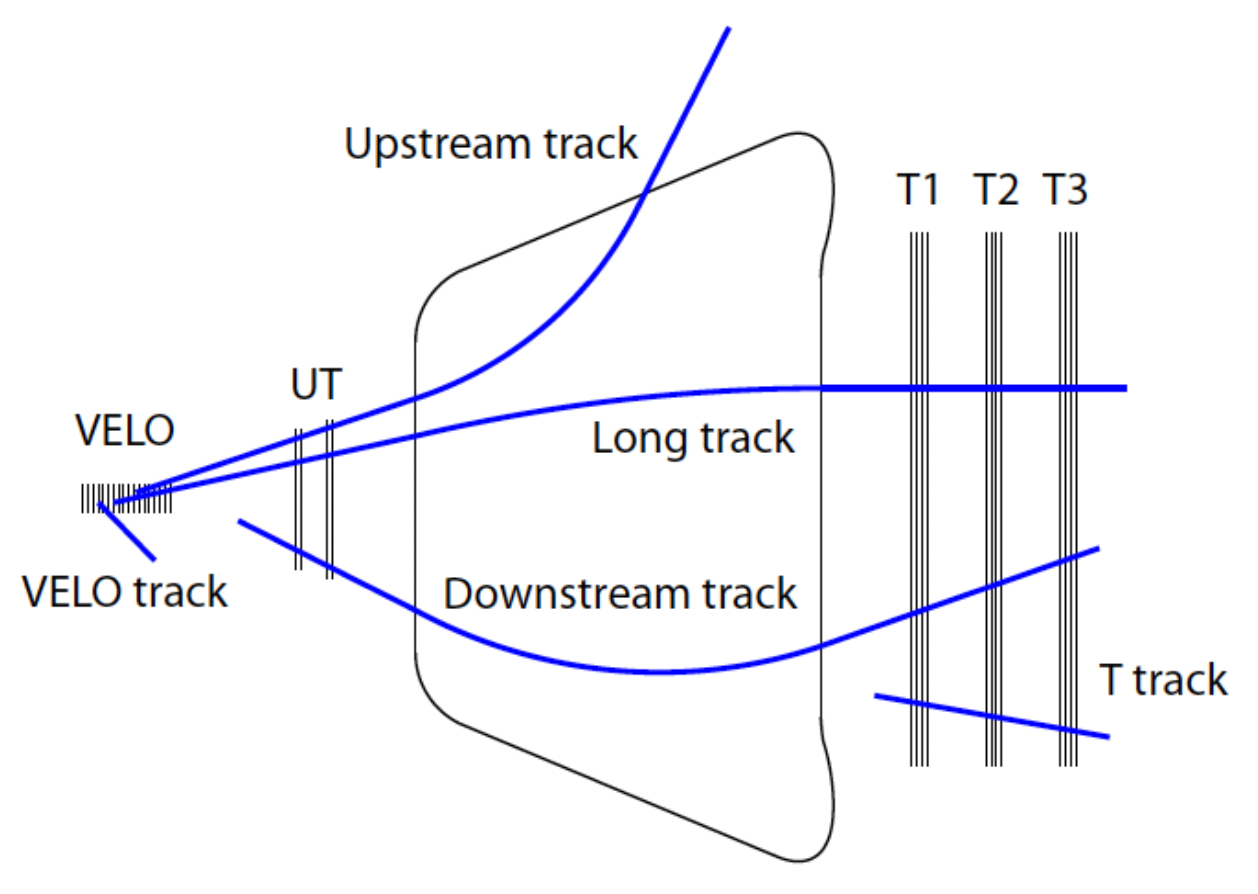
\includegraphics[width=\textwidth]{plots/track_types.png}
    \end{column}
    \begin{column}[c]{0.48\textwidth}
      \begin{itemize}
        \item $\bullet$\, Echtzeit Eventselektion
        \item $\bullet$\, Reduziert die Anzahl an fake Spuren deutlich durch matching von VELO und SciFi Spuren
        \item $\bullet$\, \to reduziert ghost Rate
        \item $\bullet$\, verbessterte Auflösung für Spuren mit kleinem Impuls \to keine oder wenige Treffer im SciFi
      \end{itemize}
    \end{column}
  \end{columns}
\end{frame}

\begin{frame}\frametitle{Scintillating Fibre Tracker (SciFi)}
  \begin{columns}
    \begin{column}[c]{0.48\textwidth}
      \begin{itemize}
        \item $\bullet$\, Letzte Element im Tracker System von LHCb
        \item $\bullet$\, 3 Stationen, 4 Schichten pro Station, 10 (12) Module pro Schicht
        \item $\bullet$\, Szintillierenden Fasern also Detektormaterial
        \item $\bullet$\, $X1-U-V-X2$ Schema with $U-V$ sterewinkel wie beim UT
        \item $\bullet$\, räumliche Auflösung: 100 $\si{\micro\metre}$
        \item $\bullet$\, Detektorfläche von 360 $\si{\metre\squared}$
      \end{itemize}
    \end{column}
    \begin{column}[c]{0.48\textwidth}
      \begin{figure}
        \centering
        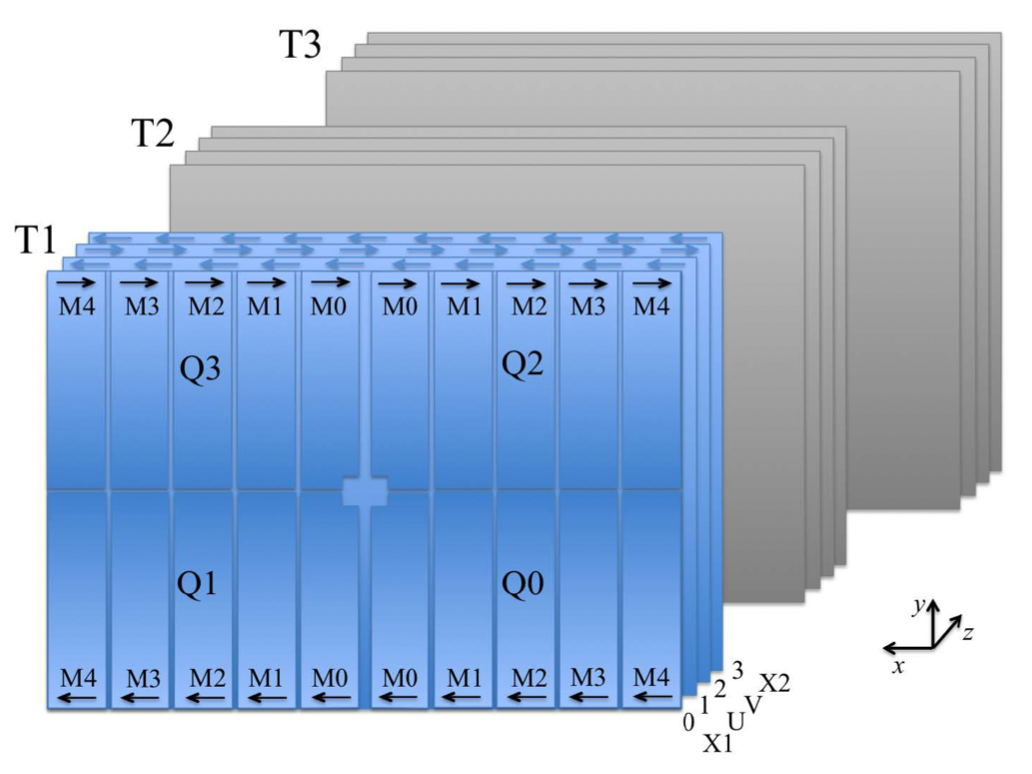
\includegraphics[width=\textwidth]{plots/scifi_layers.png}
      \end{figure}
    \end{column}
  \end{columns}
\end{frame}

\begin{frame}\frametitle{Scintillierende Fasern}
  \begin{columns}
    \begin{column}[c]{0.48\textwidth}
      \begin{itemize}
        \item $\bullet$\, Produkt: SCSF-78MJ
        \item $\bullet$\, gefärbter Styropor Kern und Wellenlängen Shifter
        \item $\bullet$\, Ummantelung mit höherem Brechungsindex für Totalreflektion innerhalb der Faser
        \item $\bullet$\, Geladene Teilchen regen $\pi$ orbitale der Benzolringe im Kernmaterial an.
        \item $\bullet$\, Relaxation führt zu szintillierendem Licht. Farbe beschleunigt den Prozess! (siehe: Förster-Transfer)
        \item $\bullet$\, Absorptions- und Emissionsspektrum so verschieden wie möglich!
        \item $\bullet$\, \to Photonen direkt wieder absorbiert \to Wellenlängenverscheiber
      \end{itemize}
    \end{column}
    \begin{column}[c]{0.48\textwidth}
      \begin{figure}
        \centering
        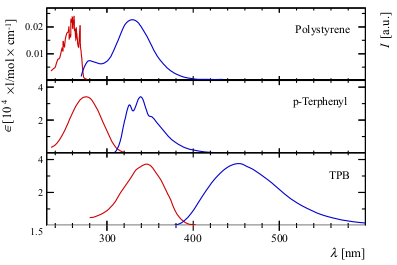
\includegraphics[width=\textwidth]{plots/shift_scifi.png}
      \end{figure}
    \end{column}
  \end{columns}
\end{frame}

\begin{frame}\frametitle{Auslese Elektronik}
  \begin{columns}
    \begin{column}[c]{0.48\textwidth}
      \begin{itemize}
        \item $\bullet$\, nur getriggerte Kanäle werden vom frontend zum backend board gesendet
        \item $\bullet$\, SiPMs senden Signal zum PACIFIC\footnote{Low Power ASIC for the SCIntillating FIbre TraCker readout} board \to digitales Signal
        \item $\bullet$\, Signale zum clustern an FPGAs senden
        \item $\bullet$\, optische Kabel zum Backend
        \item $\bullet$\, Trackbuilding ist Software Part
      \end{itemize}
    \end{column}
    \begin{column}[c]{0.48\textwidth}
      \begin{figure}
        \centering
        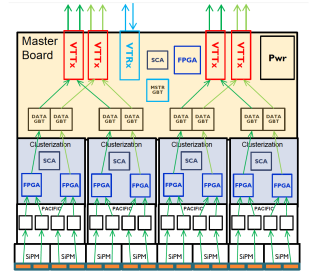
\includegraphics[width=\textwidth]{plots/readout.png}
      \end{figure}
    \end{column}
  \end{columns}
\end{frame}

\begin{frame}\frametitle{Kurzer Exkurs: FPGAs}
  \begin{columns}
    \begin{column}[c]{0.48\textwidth}
      \begin{itemize}
        \item $\bullet$\, Field Programmable Gate Arrays
        \item $\bullet$\, Integrierter Schaltkreis welcher mit logischen Schaltungen geladen werden kann.
        \item $\bullet$\, leicht rekonfigurierbar
        \item $\bullet$\, preisgünstig
        \item $\bullet$\, kurze implementierungszeiten
      \end{itemize}
    \end{column}
    \begin{column}[c]{0.48\textwidth}
      \begin{figure}
        \centering
        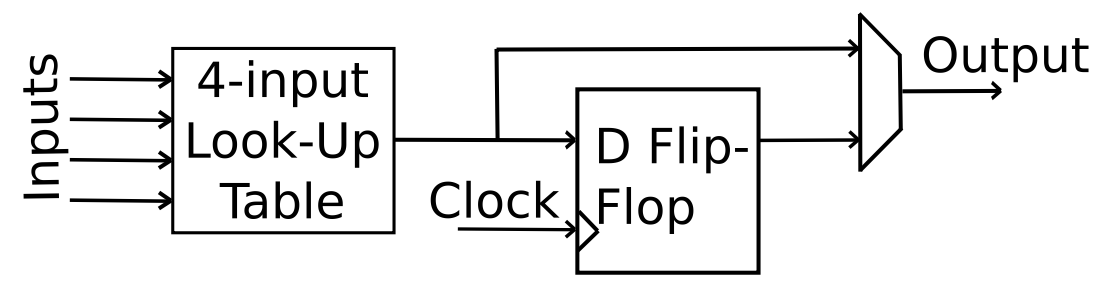
\includegraphics[width=\textwidth]{plots/FPGA.png}
      \end{figure}
    \end{column}
  \end{columns}
\end{frame}

\begin{frame}\frametitle{Why SciFi and why Fibres}
  \begin{columns}
    \begin{column}[c]{0.48\textwidth}
      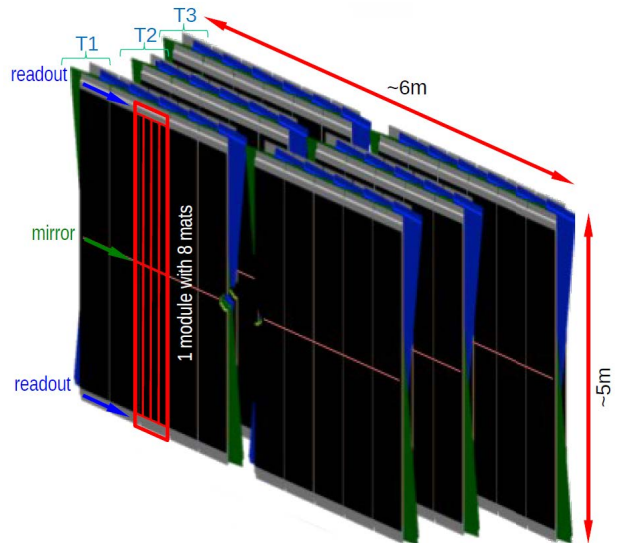
\includegraphics[width=\textwidth]{plots/scifi.png}
    \end{column}
    \begin{column}[c]{0.48\textwidth}
      \begin{itemize}
        \item $\bullet$\, szintillierende Fasern fortschrittlicher als Silizium Streifen (IT, OT)
        \item $\bullet$\, Szintillator: extrem kurze Relaxationszeit: 1 - 2 nanoseconds
        \item $\bullet$\, Ein Detektorbauteil ggü IT + OT, schnellere Reconstruktion für erhöhte Anforderungen
        \item $\bullet$\, weniger Material \to weniger Mehrfachstreuung und WW mit Materie
        \item $\bullet$\, SiPM schneller und bessere Auflösung
      \end{itemize}
    \end{column}
  \end{columns}
\end{frame}

% \begin{frame}\frametitle{Tracktypes}
%   \begin{columns}
%     \begin{column}[c]{0.48\textwidth}
%       \begin{itemize}
%         \item $\bullet$\, VELO tracks only inside VELO
%         \item $\bullet$\, Long Tracks: extended VELO Tracks matches hits in UT and SciFi
%         \item $\bullet$\, Upstream Tracks: Tracks that leave the Detector after passing the UT
%         \item $\bullet$\, Tracks without hits in the VELO
%         \item $\bullet$\, Downstream Tracks: Hits in UT and SciFi for long lived particles like Lambda and $K_s$
%         \item $\bullet$\, TTracks: only Hits in SciFi, here the seeding algorithm is used
%         \item $\bullet$\, TTracks from seeding found as long tracks by forward tracking
%         \item $\bullet$\, \to SciFi tracker has 99\% single hit efficiency
%       \end{itemize}
%     \end{column}
%     \begin{column}[c]{0.48\textwidth}
%       \begin{figure}
%         \centering
%         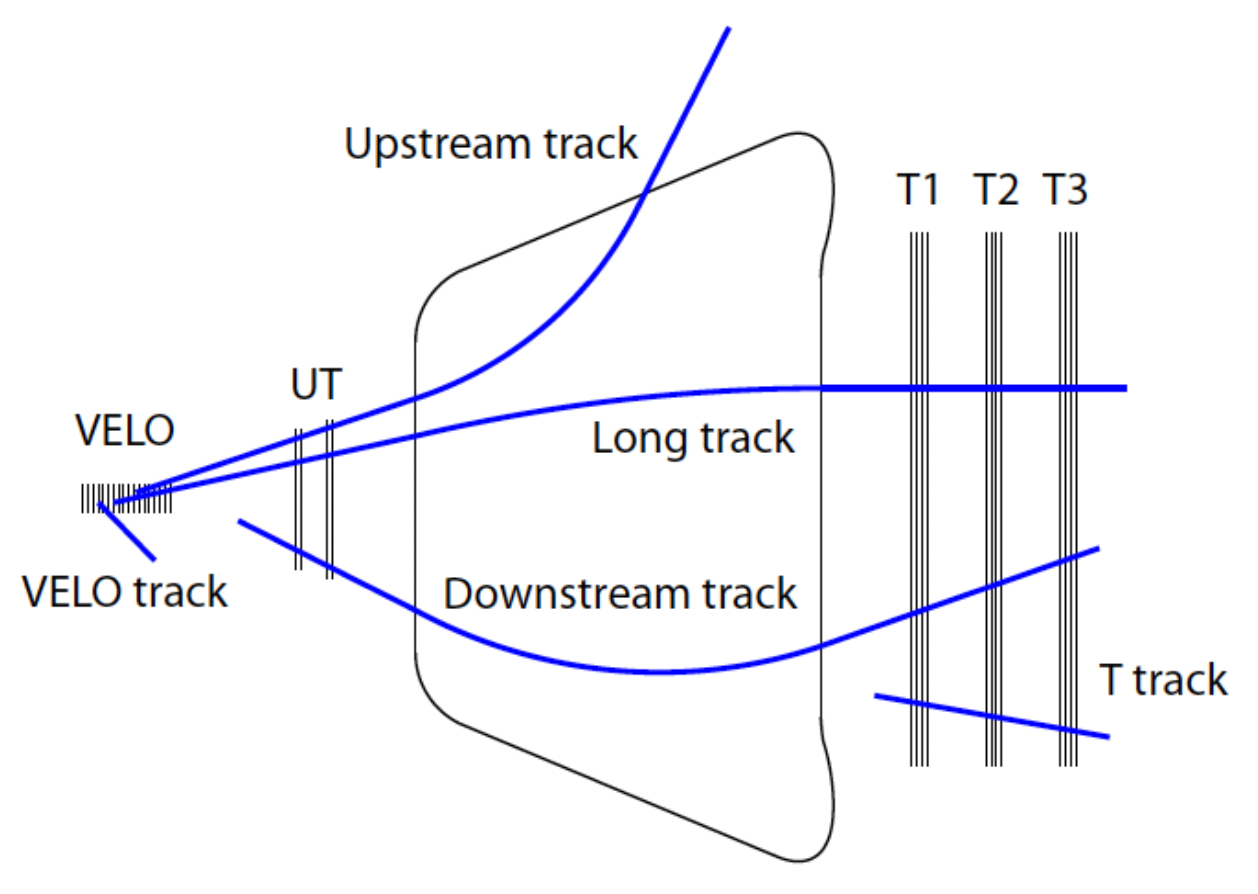
\includegraphics[width=\textwidth]{plots/track_types.png}
%       \end{figure}
%     \end{column}
%   \end{columns}
% \end{frame}

\begin{frame}\frametitle{Ring Immaging Cherenkov Detector (RICH)}
  \begin{columns}
    \begin{column}[c]{0.48\textwidth}
      \begin{itemize}
        \item $\bullet$\, PID nötig um Teilchenart zu bestimmen (Spurrekonstruktion allein genügt nicht)
        \item $\bullet$\, RICH1 downstream vom VELO, RICH2 downstream vom SciFi
        \item $\bullet$\, Cherenkov Strahlung von geladenen Teilchen
        \item $\bullet$\, SiPMs \to v der Teilchen \to rekonstruiere Masse \to PID
        \item $\bullet$\, sehr gut für: Kaonen, Pionen, Protonen
        \item $\bullet$\, RICH1 Impulsbereich: 2 - 40 $GeV/c$ for high sensitivity
        \item $\bullet$\, RICH2 Impulsbereich: 150 - 100 $GeV/c$
        \item $\bullet$\, weiter downstream: Teilchen mit hohem Impuls weniger stark abgelenkt
      \end{itemize}
    \end{column}
    \begin{column}[c]{0.48\textwidth}
      \begin{figure}
	       \centering
	       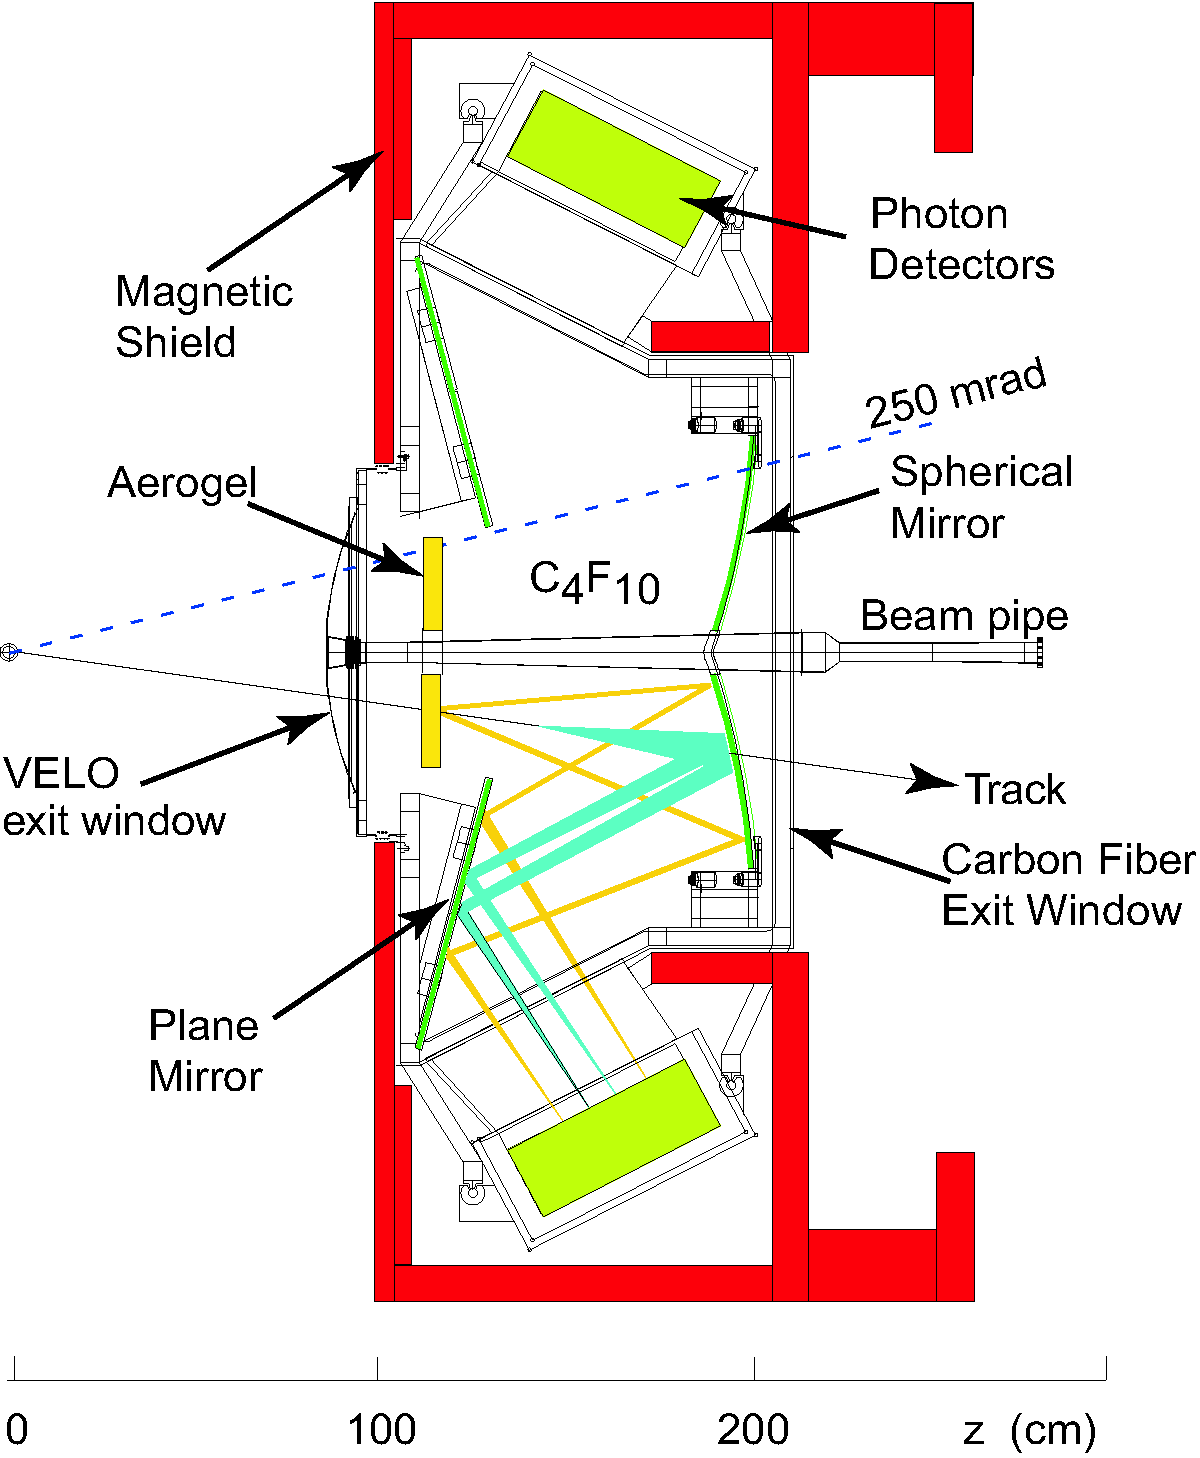
\includegraphics[width=0.8\textwidth]{plots/rich1.png}
      \end{figure}
    \end{column}
  \end{columns}
\end{frame}

\begin{frame}\frametitle{RICH2 Detector}
  \begin{columns}
    \begin{column}[c]{0.48\textwidth}
      \begin{itemize}
	       \item $\bullet$\, Kaonen threshold = 9.3 $GeV/c$
         \item $\bullet$\, Aerogel: Trennung Protonen von Kaonen aufgrund von Öffnungswinkel
         \item $\bullet$\, $\text{cos}\Theta = \frac{m}{n\cdot\beta}$
      \end{itemize}
    \end{column}
    \begin{column}[c]{0.48\textwidth}
      \begin{figure}
	       \centering
	       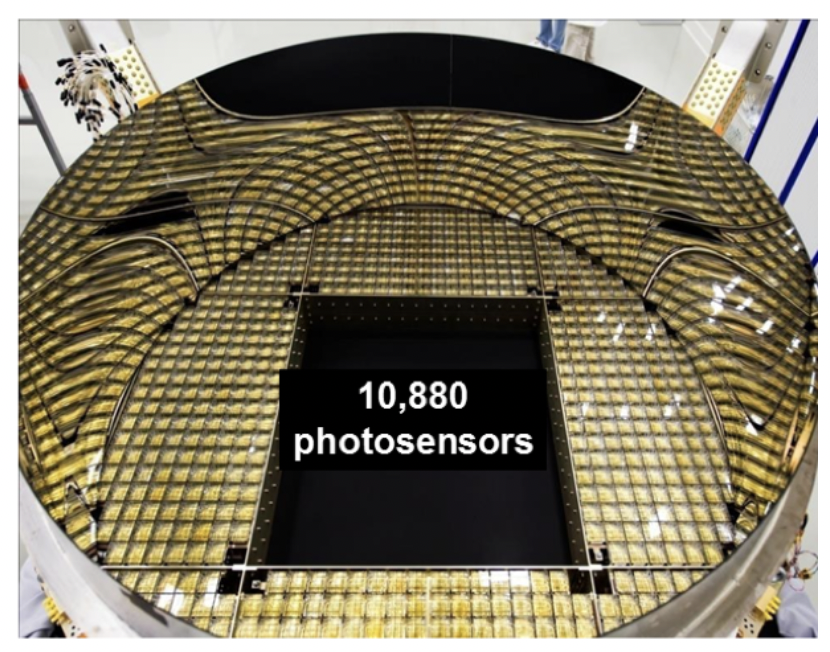
\includegraphics[width=\textwidth]{plots/rich2.png}
      \end{figure}
    \end{column}
  \end{columns}
\end{frame}

\begin{frame}\frametitle{LumiTracker: Funktion}
  \begin{columns}
    \begin{column}[c]{0.48\textwidth}
      \begin{itemize}
        \item $\bullet$\, upstream vom VELO positioniert
        \item $\bullet$\, Messung der Luminosität alle paar Sekunden benötigt
        \item $\bullet$\, muss für jeden Bunch bestimmt werden aufgrund von Variationen zwischen Bunches
        \item $\bullet$\, Precision der Ordnung 10\% minimum
        \item $\bullet$\, Maß für Detektorperformance
      \end{itemize}
    \end{column}
    \begin{column}[c]{0.48\textwidth}
      \begin{figure}
	       \centering
	       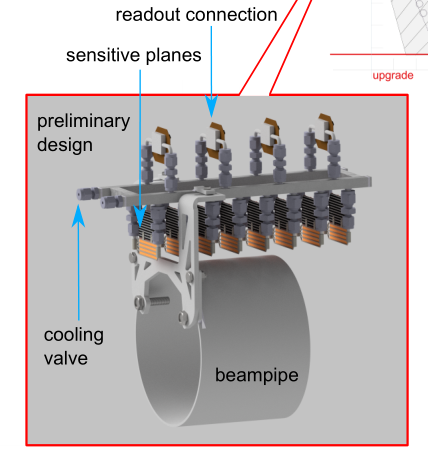
\includegraphics[width=\textwidth]{plots/lumi.png}
      \end{figure}
    \end{column}
  \end{columns}
\end{frame}

\begin{frame}\frametitle{LumiTracker: Hardware}
  \begin{columns}
    \begin{column}[c]{0.48\textwidth}
      \begin{itemize}
        \item $\bullet$\, 1 Siliziumsensor auf 3 ASICs gebaut, 6-8 Sensor Ebenen
        \item $\bullet$\, frontend "ASIC triples" mit hybrid board verkabelt (DAQ)
        \item $\bullet$\, Readout: identisch zum VELO readout
        \item $\bullet$\, Hybrid speed data links for readout, GBTx: timing und kontrollsignale
        \item $\bullet$\, OPB: für kommunikation zwischen den readout und monitor komponenten
        \item $\bullet$\, Timing Informationen: SOL40 board benutzt VeloPix ASIC codierung für software und firmware
        \item $\bullet$\, DAQ card auf remote server für spezifische messungen für den LumiTracker (lumi messung etc)
      \end{itemize}
    \end{column}
    \begin{column}[c]{0.48\textwidth}
      \begin{figure}
	       \centering
	       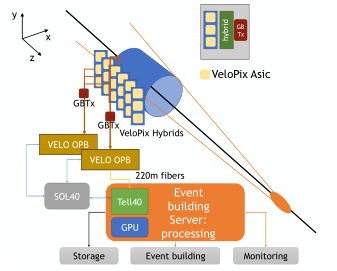
\includegraphics[width=\textwidth]{plots/lumi_design.png}
      \end{figure}
    \end{column}
  \end{columns}
\end{frame}

\begin{frame}\frametitle{LumiTracker: realization}
  \begin{columns}
    \begin{column}[c]{0.48\textwidth}
      \begin{itemize}
        \item $\bullet$\,Messung der Luminosität durch Spurzählungen durch hybrid pixel detector (VELO upgrade)
        \item $\bullet$\, $\langle \mathcal{L} \rangle = \frac{A}{\sigma_{\text{vis}}} f_r n_{\text{tracks}}$
        \item $\bullet$\, minimum 4 hits pro Spur \to linearer fit
        \item $\bullet$\, 3-hit-tracks: bessere Rekonstruktionseffizienz aber mehr Beiträge durch WW mit Materie!
      \end{itemize}
\to Vollen Detektorüberlapp mit VELO: wichtig für alignment und Kalibration
\to online bunch luminositäts Messungen: kleine Unsicherheiten (< 1\%)
    \end{column}
    \begin{column}[c]{0.48\textwidth}
      \begin{figure}
	       \centering
	       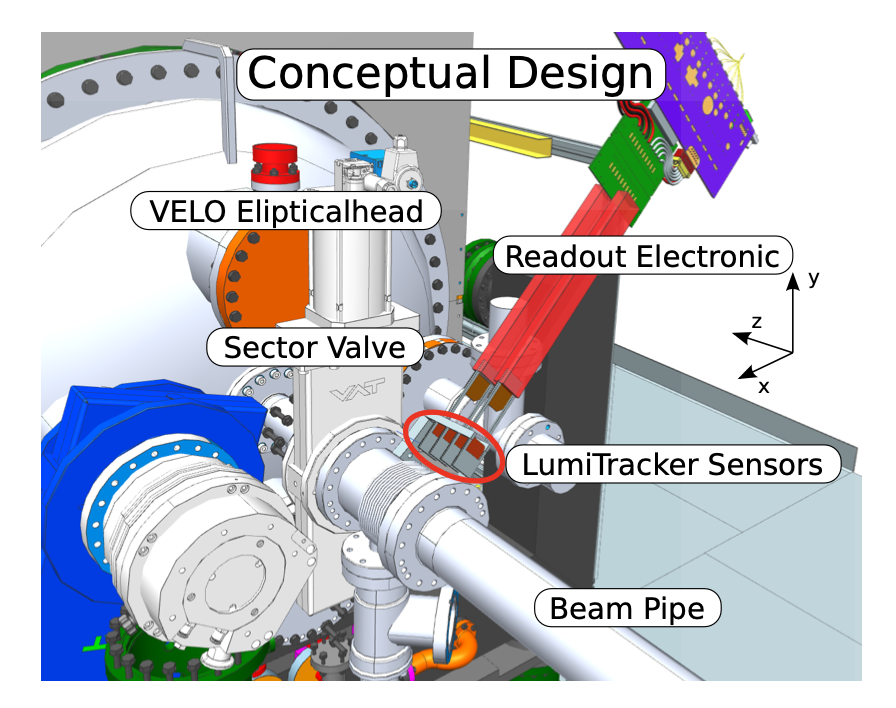
\includegraphics[width=\textwidth]{plots/lumiTracker_design.png}
      \end{figure}
    \end{column}
  \end{columns}
\end{frame}

\begin{frame}\frametitle{TimePix4 Telescope}
  \begin{columns}
    \begin{column}[c]{0.48\textwidth}
      \begin{itemize}
        \item $\bullet$\, 4 Silizium Detektorplatten pro Seite
        \item $\bullet$\, TimePix4 basierend auf readout ASIC (Art FPGA aber spezifischer auf Anwendung bezogen)
        \item $\bullet$\, Detektorplatten gegeneinander gedreht für hervorragende Ortsauflösung
        \item $\bullet$\, \to präzise Teilchenspur Rekonstruktion
        \item $\bullet$\, \approx 200 ps Zeitauflösung
      \end{itemize}
    \end{column}
    \begin{column}[c]{0.48\textwidth}
      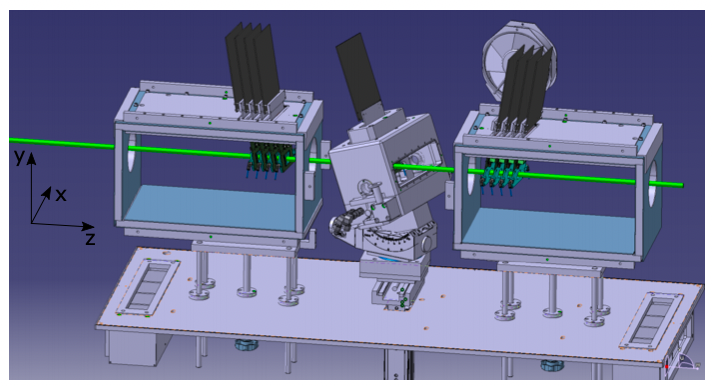
\includegraphics[width=0.5\textwidth]{plots/timepix4.png}
      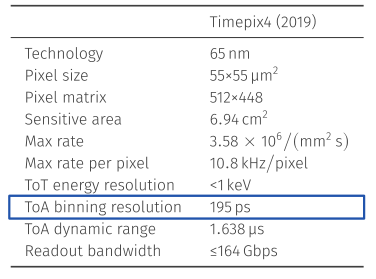
\includegraphics[width=0.5\textwidth]{plots/lumi_res.png}
    \end{column}
  \end{columns}
\end{frame}

% \begin{frame}\frametitle{}
%   \begin{columns}
%     \begin{column}[c]{0.48\textwidth}
%
%     \end{column}
%     \begin{column}[c]{0.48\textwidth}
%
%     \end{column}
%   \end{columns}
% \end{frame}

\begin{frame}\frametitle{Beam Conditions Monitor (BCM)}
  \begin{columns}
    \begin{column}[c]{0.48\textwidth}
      \begin{itemize}
        \item $\bullet$\, original: 2009 \to 2018
        \item $\bullet$\, Sicherheitsmechanismus für kritische Strahl Szenarien
        \item $\bullet$\, 2 Stationen upstream vom Magnet
        \item $\bullet$\, 8 Diamant Sensoren pro Station
        \item $\bullet$\, Simulationen nötig um kritische Situationen zu testen
      \end{itemize}
    \end{column}
    \begin{column}[c]{0.48\textwidth}
      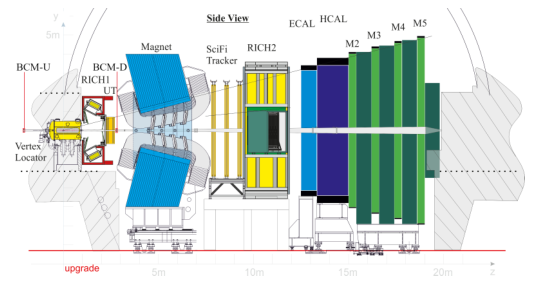
\includegraphics[width=0.8\textwidth]{plots/bcm_full.png}
    \end{column}
  \end{columns}
\end{frame}

\begin{frame}\frametitle{Diamten als Detektormaterial}
  \begin{itemize}
    \item $\bullet$\, Bethe-Bloch Formel für Energy Deposition
    \item $\bullet$\, Kristaliner Kohlenstoff, 2 ineinander verdrehte fcc gitter
    \item $\bullet$\, 43 eV um Atom aus Gitter zu entfernen
    \item $\bullet$\, Pro: mechanisch hartes Material
    \item $\bullet$\, band gap of 5.47 eV indicates insulator but can be semiconductor as well
    \item $\bullet$\, large band gap \to low number of charge carriers \to low dark current
    \item $\bullet$\, large band gap + high displcement threshold \to very radiation hard
    \item $\bullet$\, CCE picture on page 30
  \end{itemize}
\end{frame}

% \begin{frame}\frametitle{Diamonds and BCM}
%   \begin{itemize}
%     \item $\bullet$\, radiation damage \to sensors failed \to replacement of whole system
%     \item $\bullet$\, to avoid said damage in the future:
%     \item $\bullet$\, \to characterization of diamond sensors with charge collection efficiency
%   \end{itemize}
% \end{frame}

\begin{frame}\frametitle{BCM Diamant Readout (pre upgrade)}
  \begin{columns}
    \begin{column}[c]{0.48\textwidth}
      \begin{itemize}
        \item $\bullet$\, Strom ausgelesen mit CFC (current-to-frequency converter) cards
        % \item $\bullet$\, CFC cards integration time = 40 micro seconds
        \item $\bullet$\, CFC cards measurement range = (2.5 pico Amp (pA), 1 milli Amp (mA))
        \item $\bullet$\, gut für BCM Diamanten: Dunkelstrom (spontane freie Ladungsträger durch Wärme in lichtempfindlichen Halbleitern) in pico Amp Bereich und dump threshold in micro Amp Bereich
        \item $\bullet$\, digitized signal sent through redundant optical fibres with rate of 125kHz to TELL1 readout board
      \end{itemize}
    \end{column}
    \begin{column}[c]{0.48\textwidth}
      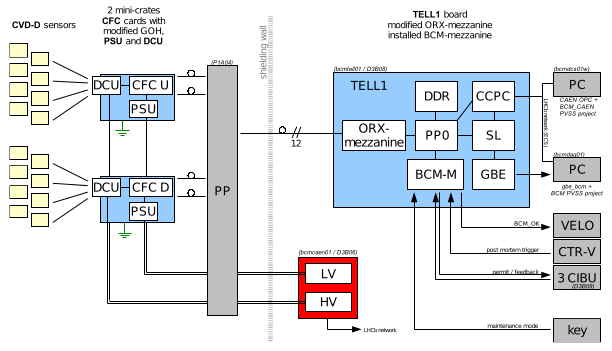
\includegraphics[width=\textwidth]{plots/bcmReadout.png}
    \end{column}
  \end{columns}
\end{frame}

\begin{frame}\frametitle{BCM Beam Dump Logic}
  \begin{columns}
    \begin{column}[c]{0.48\textwidth}
      \begin{itemize}
        \item $\bullet$\, TELL1 board: "Beam dump" wenn threshold überschritten
        \item $\bullet$\, \to langsames und schnelles Abbruchkriterium
        \item $\bullet$\, TELL1 in D3 rack hinter shielding wall in der Kaverne (CIBU interface)
        \item $\bullet$\, 2 Funktionen:
        \begin{itemize}
          \item $\bullet$\, Beam dump anfragen bei kritischen konditionen
          \item $\bullet$\, zusätzliche Bunches injizieren
        \end{itemize}
        \item $\bullet$\, post-mortem trigger: snapshot der aktuellen daten im System um nach Fehlerquellen zu suchen
        \item $\bullet$\, Signal zum VELO wenn beam kritisch
      \end{itemize}
    \end{column}
    \begin{column}[c]{0.48\textwidth}
      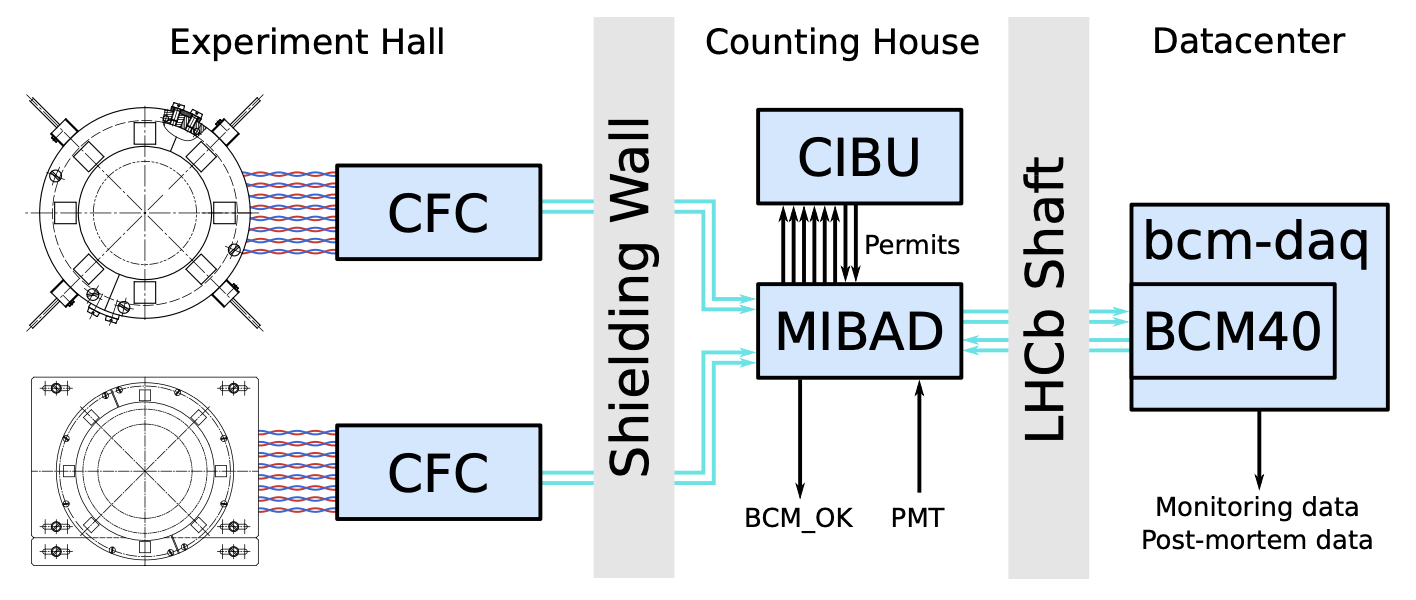
\includegraphics[width=\textwidth]{plots/data_aquisition_chain.png}
    \end{column}
  \end{columns}
\end{frame}

\begin{frame}\frametitle{BCM upgrade}
  \begin{columns}
    \begin{column}[c]{0.48\textwidth}
      \begin{itemize}
        \item $\bullet$\, 2019 \to Heute: neue Readout-Elektronik
        \item $\bullet$\, \to PCIe40 (BCM40 wird es für BCM genannt)
        \item $\bullet$\, BCM40 im Kontrollraum, CIBU Kaverne \to Transfer Bauteil nötig
        \item $\bullet$\, \to MIBAD board: Machine Interface and Beam Abort Decision board
        \item $\bullet$\, MIBAD: nutzt FPGAs für low-level Aufgaben
        \begin{itemize}
          \item $\bullet$\, implementierte beam-dump logik
          \item $\bullet$\, read-out data + post-mortem trigger
          \item $\bullet$\, VELO OK Signal
        \end{itemize}
      \end{itemize}
    \end{column}
    \begin{column}[c]{0.48\textwidth}
      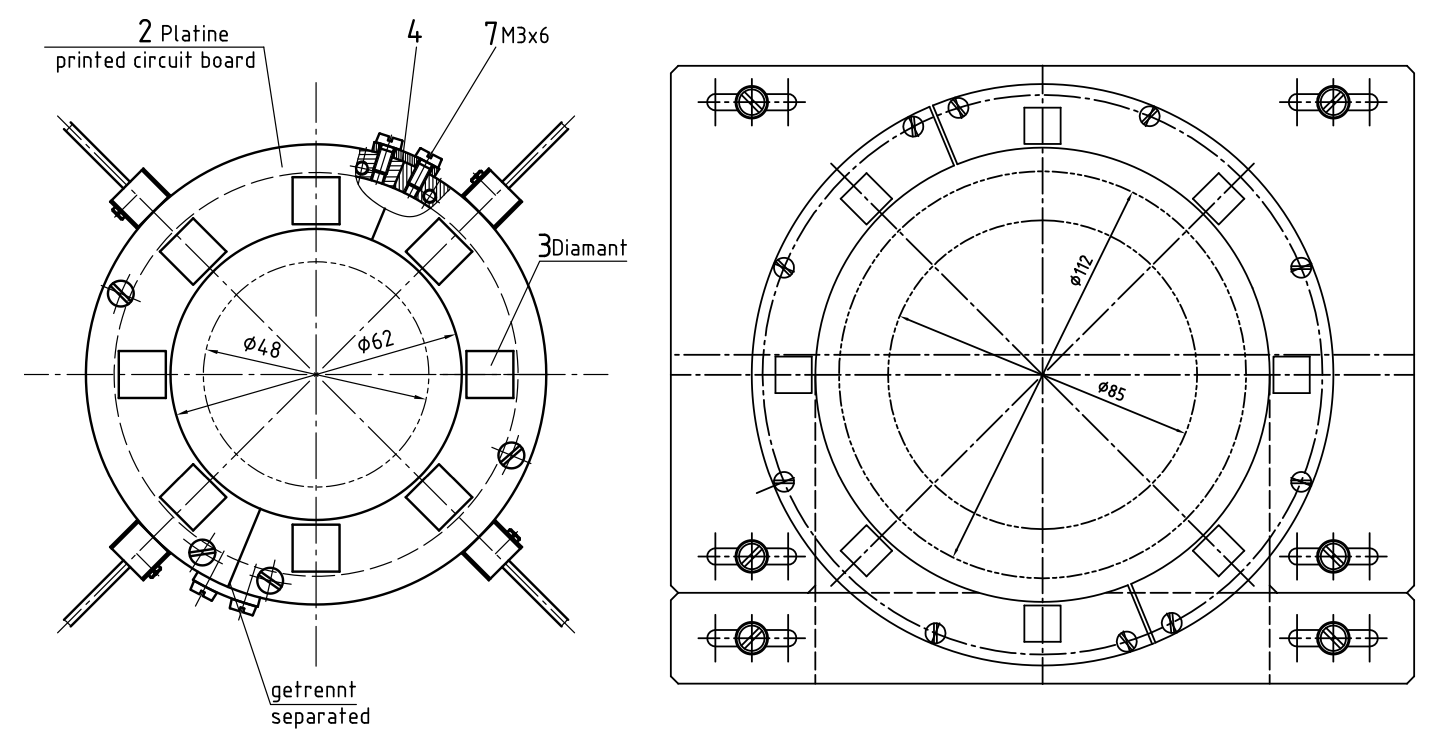
\includegraphics[width=\textwidth]{plots/BCM_U_and_BCM_D.png}
    \end{column}
  \end{columns}
\end{frame}

\begin{frame}\frametitle{BCM40 boards: Kontrollraum}
  \begin{itemize}
    \item $\bullet$\, BCM40: interface zum MIBAD board
    \item $\bullet$\, \to Kontrolle und "monitoring" des gesamten BCM
  \end{itemize}
  \to sensible Bauteile in strahlungsbelasteter Umgebung \to durchgehend unter Beobachtung
  \to BCM extrem wichtig!
\end{frame}

\end{document}
